% Define block styles
\definecolor{lightGray}{rgb}{0.97,0.97,0.97}
\definecolor{darkGray}{rgb}{0.9,0.9,0.9}
\definecolor{strokecol}{rgb}{0,0,0}
\pgfsetstrokecolor{strokecol}


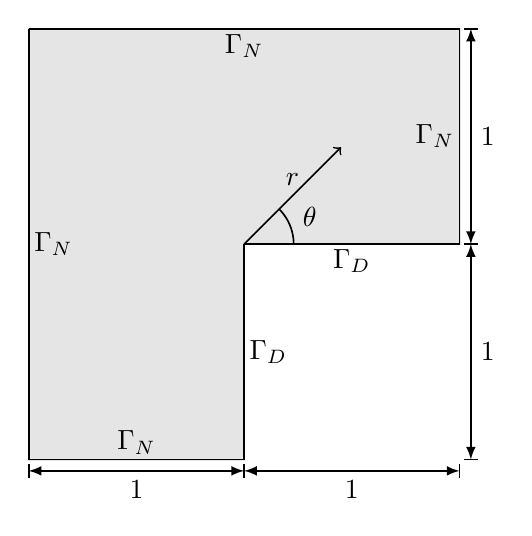
\begin{tikzpicture}[node distance = 2cm, auto, scale=0.5]
    
    \pgfsetlinewidth{0.75bp}
    %\scriptsize%        
    
    \def\width{0.95\textwidth}
    \def\rectLength{0.95*0.5*\width}

    
    
    % annular plate
    \fill[darkGray, draw=darkGray] (-\rectLength, 0) rectangle (\rectLength, \rectLength);
    \fill[darkGray, draw=darkGray] (-\rectLength, -\rectLength) rectangle (0, 0);
    
     %\draw (0,0) edge[->, draw=strokecol, fill=strokecol, semithick] (0.33*\rectLength, 0);
     %\node[] (a)  at (0.33*\rectLength, 0.08*\rectLength)  {$x$};
     %\draw  (0,0) edge[->, draw=strokecol, fill=strokecol, semithick] (0, 0.33*\rectLength);
     %\node[] (a)  at (0,0.39*\rectLength)  {$y$};
     
     \draw (0,0) edge[->, draw=strokecol, fill=strokecol, semithick] node [above] {$r$} (0.45*\rectLength, 0.45*\rectLength);
     
     \draw [draw=strokecol, semithick,domain=0:45] plot ({0.23*\rectLength*cos(\x)}, {0.23*\rectLength*sin(\x)});
     \node [ inner sep=1, outer sep=1] (theta) at ( {0.33*\rectLength*cos(22.5)} , {0.33*\rectLength*sin(22.5)} ) {$\theta$};
     
     \draw (-0,0) edge[draw=strokecol, fill=strokecol, semithick] (\rectLength, 0);
     \draw (-0,0) edge[draw=strokecol, fill=strokecol, semithick] ( 0, -\rectLength );
     
     \draw (\rectLength, 0) edge[draw=strokecol, fill=strokecol, semithick] (\rectLength, \rectLength);
     \draw (0, -\rectLength ) edge[draw=strokecol, fill=strokecol, semithick] (-\rectLength, -\rectLength);
     
	 \draw (\rectLength, \rectLength) edge[draw=strokecol, fill=strokecol, semithick] (-\rectLength, \rectLength);
     \draw (-\rectLength, -\rectLength) edge[draw=strokecol, fill=strokecol, semithick] (-\rectLength, \rectLength);
     
     % 	% BCs    
    \node [ anchor=north, inner sep=1, outer sep=1] (BC1) at ( 0 , \rectLength ) {$\Gamma_N$};
    \node [ anchor=west, inner sep=1, outer sep=1] (BC1) at ( -\rectLength, 0 ) {$\Gamma_N$};
    \node [ anchor=south, inner sep=1, outer sep=1] (BC1) at ( -0.5*\rectLength, -\rectLength ) {$\Gamma_N$};
    \node [ anchor=east, inner sep=1, outer sep=1] (BC1) at ( \rectLength, 0.5*\rectLength ) {$\Gamma_N$};
    
    \node [ anchor=north, inner sep=1, outer sep=1] (BC1) at ( 0.5*\rectLength, 0 ) {$\Gamma_D$};
    \node [ anchor=west, inner sep=1, outer sep=1] (BC1) at (
    0, -0.5*\rectLength ) {$\Gamma_D$};
    
    \draw (-\rectLength,-0.5*\width) edge[<->,>=latex,thick, draw=strokecol, fill=strokecol, semithick] node [below] {$1$} (0,-0.5*\width);
    \draw (0,-0.5*\width) edge[<->,>=latex,thick, draw=strokecol, fill=strokecol, semithick] node [below] {$1$} (\rectLength,-0.5*\width);
    
    \draw (0.5*\width,\rectLength) edge[<->,>=latex,thick, draw=strokecol, fill=strokecol, semithick] node [right] {$1$} (0.5*\width,0);
    \draw (0.5*\width,0) edge[<->,>=latex,thick, draw=strokecol, fill=strokecol, semithick] node [ right ] {$1$} (0.5*\width,-\rectLength);
%    
    \draw (0.485*\width,\rectLength) edge[draw=strokecol, fill=strokecol, semithick]  (0.515*\width, \rectLength);
    \draw (0.485*\width,0) edge[draw=strokecol, fill=strokecol, semithick]  (0.515*\width, 0);
    \draw (0.485*\width,-\rectLength) edge[draw=strokecol, fill=strokecol, semithick]  (0.515*\width,-\rectLength);
%    
     \draw (-\rectLength,-0.485*\width) edge[draw=strokecol, fill=strokecol, semithick]  (-\rectLength,-0.515*\width);
     \draw (0,-0.485*\width) edge[draw=strokecol, fill=strokecol, semithick]  (0,-0.515*\width);
     \draw (\rectLength,-0.485*\width) edge[draw=strokecol, fill=strokecol, semithick]  (\rectLength,-0.515*\width);
\end{tikzpicture}